Since the agent has access to the transition model $f$, one approach for optimizing the objective described in \secref{sec:problem} is to forgo learning entirely, and solve any held-out task by running a planner over the state state $\X$ and action space $\A$.
However, searching for a solution directly in these large spaces is highly infeasible.
Instead, we propose to \emph{learn abstractions} using the provided demonstrations.
In this section, we will describe representations that allow for fast bilevel planning with abstractions (\secref{sec:planning}).
In \secref{sec:learning}, we then describe how to learn these abstractions.

\begin{wrapfigure}{r}{0.1\textwidth}
\vspace{1em}
\hspace{-1em}
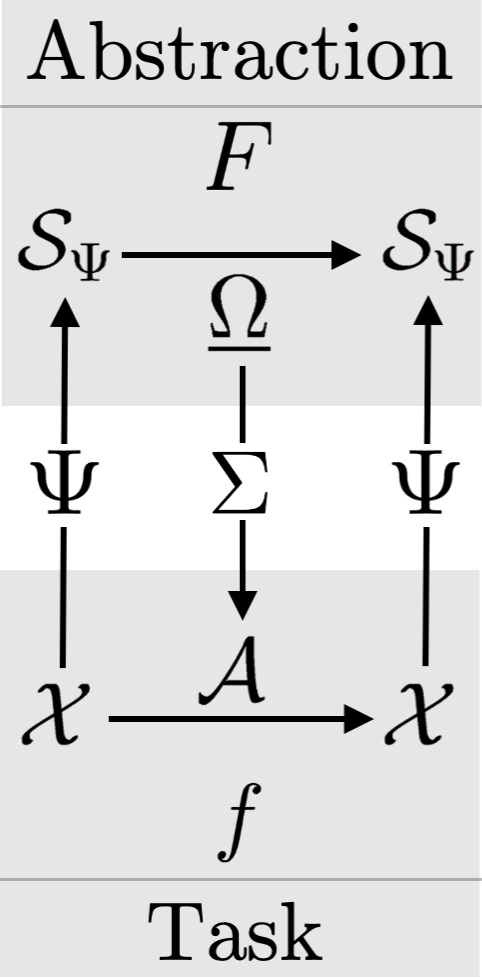
\includegraphics[width=0.1\textwidth]{figures/diagram.png}
\end{wrapfigure}

We adopt a very general definition of an abstraction~\cite{konidarisabstractions}: mappings from $\X$ and $\A$ to alternative state and action spaces. 
We first characterize an abstract state space $\S_\Psi$ and a transformation from states in $\X$ to abstract states.
Next, we describe an abstract action space $\ground{\operators}$ and an abstract transition model $F : \S_\Psi \times \ground{\operators} \to \S_\Psi$ that can be used to plan in the abstract space.
Finally, we define samplers $\samplers$ for refining abstract actions back into $\A$, i.e., actions that can be executed. See the diagram on the right for a summary.

\textbf{(1) An abstract state space.}
We use a set of predicates $\Psi$ (as defined in \secref{sec:problem}) to induce an abstract state space $\S_\Psi$.
Recalling that a ground atom $\ground{\psi}$ induces a classifier $c_{\ground{\psi}}$ over states $x \in \X$, we have:
\begin{defn}[Abstract state]
An \emph{abstract state} $s$ is the set of ground atoms under $\Psi$ that hold true in $x$: $$s = \textsc{Abstract}(x, \Psi) \triangleq \{ \ground{\psi} : c_{\ground{\psi}}(x) = \text{\emph{true}}, \forall \psi \in \Psi \}.$$
\end{defn}
The (discrete) abstract state space induced by $\Psi$ is denoted $\S_{\Psi}$.
Throughout this work, we use predicate sets $\Psi$ that are supersets of the given goal predicates $\Psi_G$.
However, only the goal predicates are given, and they alone are typically very limited; in \secref{sec:learning}, we will discuss how the agent can use data to \emph{invent predicates} that will make up the rest of $\Psi$. See \figref{fig:teaser} (first panel) for an example.


\textbf{(2) An abstract action space and abstract transition model.} We address both by having the agent learn \emph{operators}:

\begin{defn}[Operator]
An \emph{operator} is a tuple $\operator = \langle \params, \preconditions, \addeffects, \deleteeffects, \controllerspec \rangle$ where:
\begin{tightlist}
\item $\params$ is an ordered list of \emph{parameters}: variables with types drawn from the type set $\types$.
\item $\preconditions, \addeffects, \deleteeffects$ are \emph{preconditions}, \emph{add effects}, and \emph{delete effects}, each a set of lifted atoms over $\Psi$ and $\params$. 
\item $\controllerspec$ is a tuple $\langle C, \params_{\controllerspec} \rangle$ where $C((\type_1, \dots, \type_v), \Theta)$ is a controller and $\params_{\controllerspec}$ is an ordered list of \emph{controller arguments}, each a variable from $\params$. Furthermore, $|\params_{\controllerspec}| = v$, and each argument $i$ must be of the respective type $\type_i$.
\end{tightlist}
\end{defn}

We denote the set of operators as $\Omega$.
See \figref{fig:teaser} (second panel) for an example. Unlike in STRIPS~\cite{fikes1971strips}, our operators are augmented with controllers and controller arguments, which will allow us to connect to the task actions in \textbf{(3)} below. Now, given a task with object set $\O$, the set of all \emph{ground operators} defines our (discrete) abstract action space for a task:

\begin{defn}[Ground operator / abstract action]
A \emph{ground operator} $\ground{\operator} = \langle \operator, \delta \rangle$ is an operator $\operator$ and a substitution $\substitution : \params \to \O$ mapping parameters to objects.
We use $\ground{\preconditions}, \ground{\addeffects}, \ground{\deleteeffects}$, and $\ground{\params_{\controllerspec}}$ to denote the ground preconditions, ground add effects, ground delete effects, and ground controller arguments of $\ground{\operator}$, where variables in $\params$ are substituted with objects under $\substitution$.
\end{defn}

We denote the set of ground operators (the abstract action space) as $\ground{\operators}$. Together with the abstract state space $\S_\Psi$, the preconditions and effects of the operators induce an abstract transition model for a task:

\begin{defn}[Abstract transition model]
\label{def:absmodel}
The \emph{abstract transition model} induced by predicates $\Psi$ and operators $\operators$ is a partial function $F : \S_\Psi \times \ground{\operators} \to \S_\Psi$. $F(s, \ground{\operator})$ is only defined if $\ground{\operator}$ is \emph{applicable} in $s$:  $\ground{\preconditions} \subseteq s$. If defined, $F(s, \ground{\operator}) \triangleq (s - \ground{\deleteeffects}) \cup \ground{\addeffects}$.
\end{defn}

\textbf{(3) A mechanism for refining abstract actions into task actions.} A ground operator $\ground{\operator}$ induces a partially specified controller, $C((o_1, \ldots o_v), \Theta)$ with $(o_1, \ldots o_v) = \ground{\params_{\controllerspec}}$, where object arguments have been selected but continuous parameters $\Theta$ have not. To \emph{refine} this abstract action $\ground{\operator}$ into a task-level action $a = C((o_1, \ldots o_v), \theta)$, we use \emph{samplers}:

\begin{defn}[Sampler]
Each operator $\operator \in \operators$ is associated with a \emph{sampler} $\sampler : \X \times \O^{|\params|} \to \Delta(\Theta)$, where $\Delta(\Theta)$ is the space of distributions over $\Theta$, the continuous parameters of the operator's controller.
\end{defn}

\begin{defn}[Ground sampler]
For each ground operator $\ground{\operator} \in \ground{\operators}$, if $\ground{\operator} = \langle \operator, \delta \rangle$ and $\sampler$ is the sampler associated with $\operator$, then the $\emph{ground sampler}$ associated with $\ground{\operator}$ is a state-conditioned distribution $\ground{\sampler} : \X \to \Delta(\Theta)$, where $\ground{\sampler}(x) \triangleq \sampler(x, \delta(\params))$.
\end{defn}

We denote the set of samplers as $\samplers$. See \figref{fig:teaser} (third panel) for an example.

What connects the transition model $f$, abstract transition model $F$, and samplers $\samplers$? While previous works enforce the downward refinability property~\cite{marthi2007angelic,pasula2007learning,jetchev2013learning,konidaris2018skills}, it is important in robotics to be robust to violations of this property, since learned abstractions will typically lose critical geometric information.
Therefore, we only require our learned abstractions to satisfy the following \emph{weak semantics}:
for every ground operator $\ground{\operator}$ with partially specified controller $C((o_1, \dots, o_v), \Theta)$ and associated ground sampler $\ground{\sampler}$, there exists some $x \in \X$ and some $\theta$ in the support of $\ground{\sampler}(x)$ such that $F(s, \ground{\operator})$ is defined and equals $s'$, where $s = \textsc{Abstract}(x, \Psi)$, $a = C((o_1, \dots, o_v), \theta)$, and $s' = \textsc{Abstract}(f(x, a), \Psi)$.
Note that downward refinability~\cite{marthi2007angelic} makes a much stronger assumption: that this statement holds for \emph{every} $x \in \X$ where $F(s, \ground{\operator})$ is defined.